\section{System Design}
\label{sec:system}

This section presents the detailed system design of \name.% to realize the two design choices presented in \Section\ref{sec:overview}.

\subsection{\name architecture}
\label{subsec:system:architecture}

\begin{figure}[t]
  \centering
  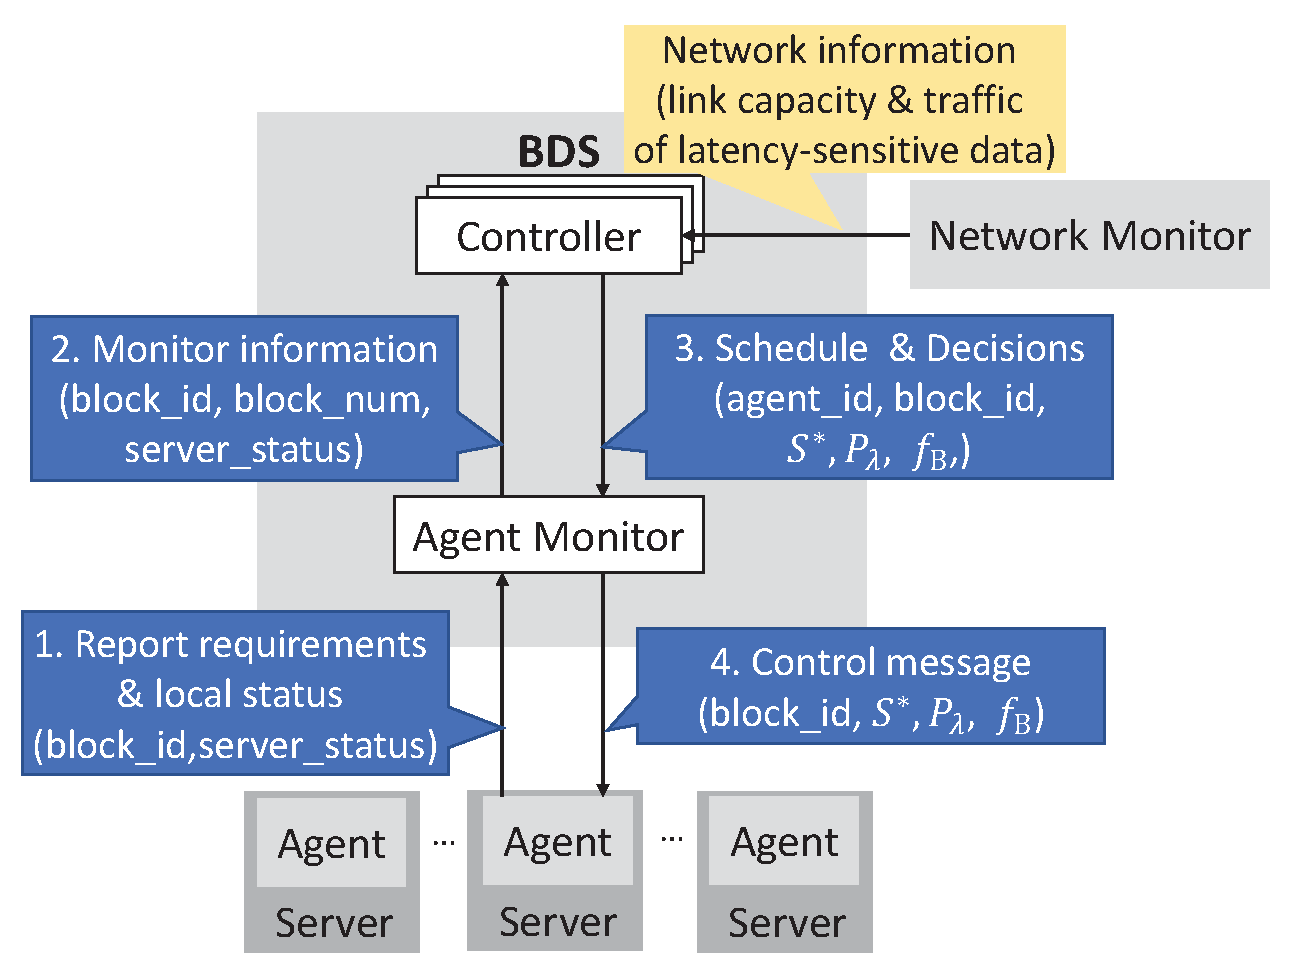
\includegraphics[width=3in]{images/implementation_v2.eps}
  \tightcaption{The implementation of \name.}
  \label{fig:implementation}
\vspace{-0.4cm}
\end{figure}
%\vspace{-15pt}

\name reuses the same underlying multicast system described in \Section\ref{subsec:motivation:case-for}. Figure \ref{fig:implementation} shows the detailed architecture of \name. It consists of four components: Controller, Agent Monitor, Agent, Network Monitor. (1) \emph{Controller} is a scheduler which executes the customized scheduling algorithm. (2) \emph{Agent Monitor} delivers messages between the \emph{Controller} and \emph{Agents}. (3) \emph{Agent} is a module deployed in each node. It announces the bulk data download requirement to the agent monitor and triggers the transmission on local nodes. (4) \emph{Network Monitor} monitors the aggregated traffic of latency-sensitive data and maintains each link's capacity, which are the basic inputs of the scheduling algorithm.

\subsection{Centralized control}
\label{subsec:system:centralized}

The centralized controller of \name sets a 3-second scheduling cycle and updates the scheduling results in each cycle. The control level interfaces are implemented by HTTP POST (including: 1. the data collection process from agents to the controller, and 2. the control messages updating process from the controller to agents). Specifically, the basic workflow in one cycle can be described as follows: (1) the local agent on each node checks the block status, records the ids of blocks that finished downloading in this cycle, and then reports the status and information to the agent monitor. (2) Agent Monitor aggregates the information from all the agents, updates block duplication status, and sends the updated information to the controller. (3) the controller runs the centralized scheduling algorithm, works out the near-optimal scheduling and routing results, and then sends them to the agent monitor. (4) agent monitor then forwards the control messages back to the corresponding local agents. (5) the local agent sets the transmission rate according to the received control message, then uses \emph{wget} tools to download the bulk data.
%\jc{the para needs a clearer message: how centralized control is implemented? what's the data collection interface? what's the control interface? Don't use mathmatical notations (again don't assume people have read section 4) or protocols like http post (they belong to implementation).}

There are two further optimizations when implementing centralized control.
\begin{itemize}
\item \emph{Merging blocks}. \name merges the blocks with the same source and destination pair into one subtask. There are two objectives. The first one is to reduce the computation scale and the second one is to achieve higher-efficient transmissions. Without this merging process: 1) there will be a large number of pending tasks in the next scheduling cycle, making calculation computationally hard to finish within an acceptable time; 2) all blocks will establish their connections at the same time, sharing the limited server rate, thus cannot be finished and will be hung up for the next cycle, resulting in inefficient transmissions.
\item \emph{Non-blocking update}. No matter how fast the controller runs, it still takes some time to work out the scheduling and routing solutions in each cycle. During this algorithm running time, \name continues the transmissions according to the configurations in the last cycle instead of pausing transfers and waiting for new configurations. To ensure consistency, the controller will estimate the task status after the algorithm running time and use this future status as inputs of the scheduling algorithm.
\end{itemize}

%\begin{itemize}
%
%\item Start with the basic workflow of each 3-second cycle: (1) how local agent collects delivery status, (2) send messages to the controller, (3) controller runs the algorithm, (4) control message to each local agent, and (5) how local agent enforce decision.
%
%\item Fault tolerance: what if a server is not available (or straggling), what if one controller instance is not available, what if there is network partition between DCs or between DCs and the controller.
%
%\item Explain two optimizations:
%\begin{itemize}
%\item Merging blocks
%\item Non-blocking update
%\end{itemize}
%
%\end{itemize}

\subsection{Dynamic bandwidth separation}
\label{subsec:system:separation}

To guarantee dynamic bandwidth separation between bulk data and the delay-sensitive user data, \name monitors all the latency-sensitive traffic according to source IPs, then aggregates traffic on all the inter-/intra-DC links in real time.

With the known link capacity and the aggregated size of latency-sensitive traffic, the residual bandwidth for background data can then be calculated by the difference of the two. So the upper bound for the available bandwidth of all links are all confirmed in the scheduling algorithm. In the server end, each agent enforces the bandwidth limits by Linux Traffic Control (TC). Thus, \name achieves the bandwidth separation dynamically and in real-time.

Such dynamic bandwidth separation scheme is different from the traditional priority-based techniques (such as \cite{kumar2015bwe}), which sets higher priority to online latency-sensitive traffic than background traffic. When traffic bursts, such priority-based techniques still work as usual by allocating bandwidth according to traffic priorities, ignoring whether the online traffic is suffering from high latency. While this can be avoided by \name, which dynamically monitors the occupied bandwidth by delay-sensitive applications and reservers enough bandwidth for them, and thus is able to guarantee the performance of latency-sensitive applications.


%\jc{please put this solution into context. what's the diff to priority-based techniques such as bwe?}


\subsection{Fault Tolerance}
\label{subsec:system:fault}
To make \name fault tolerant, the following scenarios are also considered.

\begin{packedenumerate}
\item \emph{What if the controller is not available?} The controller is replicated three times for fault recovery. Once the master controller fails, one replica will be brought up via distributed consensus protocols, such as \cite{lamport1998part}.
\item \emph{What if a server is not available (or straggling)?} If the agent on this server is still able to work, it will report the abnormal server state to the agent monitor. Otherwise, the server that has selected this server as data source would report the invalid status to the agent monitor. In both cases, the controller would remove that server from the potential data sources in the next scheduling cycle.
\item \emph{What if there is network partition between DCs or between DCs and the controller?} If network partition happens between DCs and the controller, the whole network will reverse to a default decentralized overlay protocol to ensure graceful degradation on performance. If network partition happens between DCs, then the DCs that locate in the same partition with the controller will work the same as before, while the separated DCs will downgrade to the default decentralized overlay network.
\end{packedenumerate}
%
%\begin{itemize}
%
%\item First, how to get real-time aggregated size of latency-sensitive traffic.
%
%\item Second, how to calculate the bandwidth cap for background bulk traffic
%
%\item Finally, how to enforce the bandwidth cap.
%
%\end{itemize}



